\begin{figure}[H]
\centering
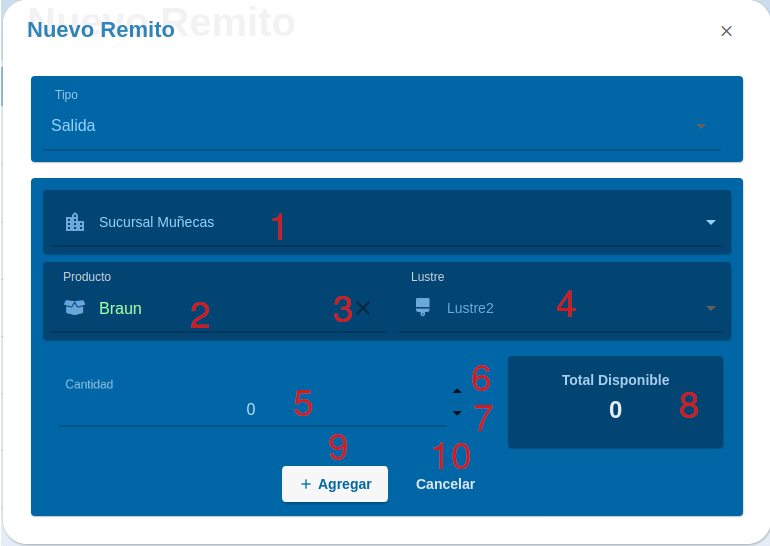
\includegraphics[width=\textwidth,height=\textheight,keepaspectratio]{Escenarios/AD-18-00}
\caption{Escenario - AD-18-00}
\label{fig:AD-18-00}
\end{figure}
Este es el escenario que permite a los usuarios crear o modificar líneas de remito. La lista desplegable \textbf{AD-18-01} aparecerá en caso de estar creando una linea de remito para un remito de salida. En el campo \textbf{AD-18-01} el usuario indicará el producto con el cual se está creando o bien el nuevo producto en caso de estar modificando. El botón \textbf{AD-18-03} permite eliminar la selección del campo \textbf{AD-18-02}. La lista desplegable \textbf{AD-18-04} le permite al usuario seleccionar el lustre deseado. El campo \textbf{AD-18-05} indica la cantidad de producto elegido, con un click en los botones \textbf{AD-18-06} y \textbf{AD-18-07} se incrementa y se decrementa una unidad del campo \textbf{AD-18-05} respectivamente. El campo\textbf{AD-18-08}, se automcompletará con la cantidad disponible del producto en la ubicación seleccionada en el campo \textbf{AD-18-01}, en caso de tratarse de un remito de salida. 
Un click en el botón \textbf{AD-18-09} creará o modificará la linea de remito y navegará al escenario \textbf{AD-17-00}, mientras que un click en el botón \textbf{AD-18-10} descartará todos los cambios realizados y navegará al escenario \textbf{AD-17-00}.
\clearpage
